\documentclass[a4paper,12pt,titlepage]{article}
\usepackage{amsmath} 
\usepackage{amssymb}
\usepackage[nottoc]{tocbibind}
\usepackage{float}
\usepackage{indentfirst}
\author{\textit{Jiang Yicheng}\\\textit{515370910224}}
\title{\textbf{VV286\\ Honors Mathematics IV\\
Ordinary Differential Equations\\
		Assignment 3}}
\date{\today}
\usepackage{extarrows}
\usepackage{dsfont}
\usepackage[top=1 in, bottom=0.8 in, left= 1in, right=1 in]{geometry}
\usepackage{fancyhdr,lastpage}
	\pagestyle{fancy}
	\fancyhf{}
\cfoot{Page \thepage\ of \pageref{LastPage}}
\usepackage{multirow}
\usepackage{gauss}
\usepackage{geometry}
\usepackage{graphicx}
\begin{document}

\maketitle

\section{}
\subsection{}
\paragraph{Proof:}$\forall \varphi(x)=e^{-x^2/2}p(x)\in V$,
\begin{align*}
H\varphi=&-\dfrac{d^2}{dx^2}e^{-x^2/2}p(x)+x^2e^{-x^2/2}p(x)\\
=&-\dfrac{d}{dx}(e^{-x^2/2}\cdot(-x)p(x)+e^{-x^2/2}p'(x))+x^2e^{-x^2/2}p(x)\\
=&e^{-x^2/2}\cdot(-x)xp(x)+e^{-x^2/2}(p(x)+xp'(x))\\
&-(e^{-x^2/2}\cdot(-x)p'(x)+e^{-x^2/2}p''(x))+x^2e^{-x^2/2}p(x)\\
=&e^{-x^2/2}(p(x)+2xp'(x)-p''(x))
\end{align*}

Since $p(x)\in\mathcal{P}(\mathbb{R})$, $p(x)+2xp'(x)-p''(x)\in\mathcal{P}(\mathbb{R})$. So $H\varphi\in V$.

So $H\varphi\in V$ if $\varphi\in V$.
\subsection{}
$\forall \varphi(x)=e^{-x^2/2}p_1(x)\in V,\psi(x)=e^{-x^2/2}p_2(x)\in V$,
\begin{align*}
&\langle H\psi,\varphi\rangle-\langle \psi,H\varphi\rangle\\
=&\int_{-\infty}^{\infty}H\psi\cdot\varphi dx-\int_{-\infty}^{\infty}\psi\cdot H\varphi dx\\
=&\int_{-\infty}^{\infty}e^{-x^2/2}(p_2(x)+2xp'_2(x)-p''_2(x))\cdot e^{-x^2/2}p_1(x)dx\\
&-\int_{-\infty}^{\infty}e^{-x^2/2}p_2(x)\cdot e^{-x^2/2}(p_1(x)+2xp'_1(x)-p''_1(x))  dx\\
=&\int_{-\infty}^{\infty}e^{-x^2}(2xp_1(x)p'_2(x)-p_1(x)p''_2(x)-2xp'_1(x)p_2(x)+p_2(x)p''_1(x))dx\\
=&e^{-x^2}(p'_1(x)p_2(x)-p_1(x)p'_2(x))\Big|_{-\infty}^{\infty}
\end{align*}
Since $p_1(x),p_2(x)\in\mathcal{P}(\mathbb{R})$, then use L'Hopital's rule we can get that $$\underset{x\rightarrow \pm\infty}{lim}e^{-x^2}p'_1(x)p_2(x)=\underset{x\rightarrow \pm\infty}{lim}e^{-x^2}p_1(x)p'_2(x)=0$$
so $\langle H\psi,\varphi\rangle=\langle \psi,H\varphi\rangle$, i.e. $H$ is symmetric.

\subsection{}
$\forall \varphi(x)=e^{-x^2/2}p(x)\in V,$,
\begin{align*}
&(HA-AH)\varphi-2A\varphi\\
=&((-\dfrac{d^2}{dx^2})+x^2)(-\dfrac{d}{dx}+x)e^{-x^2/2}p(x)-(-\dfrac{d}{dx}+x)((-\dfrac{d^2}{dx^2})+x^2)e^{-x^2/2}p(x)\\
&-2(-\dfrac{d}{dx}+x)e^{-x^2/2}p(x)
\end{align*}

\begin{align*}
=&((-\dfrac{d^2}{dx^2})+x^2)(-(e^{-x^2/2}(-x)p(x)+e^{-x^2/2}p'(x))+xe^{-x^2/2}p(x))\\
&-(-\dfrac{d}{dx}+x)(e^{-x^2/2}(p(x)+2xp'(x)-p''(x)))\\
&-2(-(e^{-x^2/2}(-x)p(x)+e^{-x^2/2}p'(x))+xe^{-x^2/2}p(x))\\
=&e^{-x^2/2}(2xp(x)-p'(x)+2x(2xp(x)-p'(x))'-(2xp(x)-p'(x))'')\\
&+e^{-x^2/2}(-xp(x)-2x^2p'(x)+xp''(x)+p'(x)+2p'(x)+2xp''(x)-p'''(x))\\
&-e^{-x^2/2}(xp(x)+2x^2p'(x)-xp''(x))-2e^{-x^2/2}(2xp(x)-p'(x))\\
=&e^{-x^2/2}(6xp(x)+(4x^2-5)p'(x)-4xp''(x)+p'''(x))\\
&+e^{-x^2/2}(-xp(x)+(-2x^2+3)p'(x)+3xp''(x)-p'''(x))\\
&+e^{-x^2/2}(-5xp(x)+(-2x^2+2)p'(x)+xp''(x))\\
=&0
\end{align*}
So $(HA-AH)\varphi=2A\varphi$ for all $\varphi\in V$. So $[H,A]=HA-AH=2A$.

\subsection{}
Since $\psi\in V $ is an eigenfunction of $H$ for the eigenvalue $\lambda\in\mathbb{R}$, 
$$H\psi=\lambda\psi$$
then 
\begin{align*}
H(A\psi)=2A\psi+AH\psi=2A\psi+A(\lambda\psi)=2A\psi+\lambda A\psi=(\lambda+2)A\psi
\end{align*}

So $A\psi$ is an eigenfunction of $H$ for the eigenvalue $\lambda+2$.


\subsection{}
$H_0(x)=(-1)^0e^{x^2}e^{-x^2}=1$

$H_1(x)=(-1)^1e^{x^2}\dfrac{d}{dx}e^{-x^2}=-e^{x^2}\cdot e^{-x^2}\cdot(-2x)=2x$

$H_2(x)=(-1)^2e^{x^2}\dfrac{d^2}{dx^2}e^{-x^2}=e^{x^2}\dfrac{d}{dx} (e^{-x^2}\cdot(-2x))=-2e^{x^2}\cdot e^{-x^2}((-2x)x+1)=4x^2-2$

\begin{figure}[H]
    \centering
    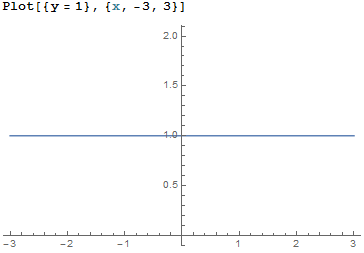
\includegraphics[width=7cm]{1.png}
    \caption{Figure for $H_0(x)=1$}
\end{figure}

\begin{figure}[H]
    \centering
    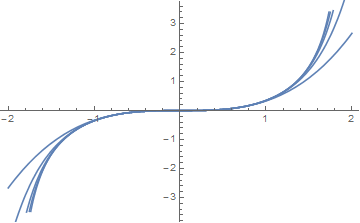
\includegraphics[width=8cm]{2.png}
    \caption{Figure for $H_1(x)=2x$}
\end{figure}
\begin{figure}[H]
    \centering
    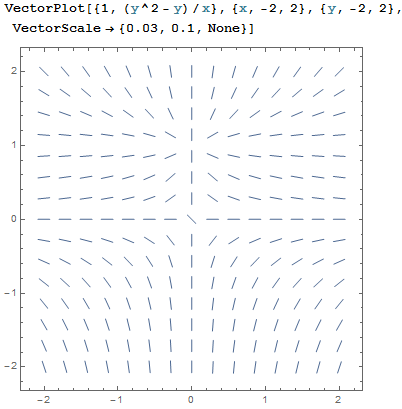
\includegraphics[width=8cm]{3.png}
    \caption{Figure for $H_2(x)=4x^2-2$}
\end{figure}

\subsection{}
$$H(e^{-x^2/2})=e^{-x^2/2}(1+2x\cdot\dfrac{d1}{dx}-\dfrac{d^21}{dx^2})=e^{-x^2/2}$$
\begin{align*}
e^{x^2/2}\Big(-\dfrac{d}{dx}\Big)(e^{-x^2/2}f(x))&=-e^{x^2/2}\cdot(e^{-x^2/2}(-x)f(x)+e^{-x^2/2}f'(x))\\&
=xf(x)+\dfrac{d}{dx}f(x)\\
&=Af(x)
\end{align*}
So $H(e^{-x^2/2})=e^{-x^2/2},Af(x)=e^{x^2/2}\Big(-\dfrac{d}{dx}\Big)(e^{-x^2/2}f(x))$.

Use induction to prove that $\psi_n(x)=e^{-x^2/2}H_n(x)$ is eigenfunctions of $H$ to eigenvalues $\lambda_n=2n+1,n\in\mathbb{N}$
\begin{enumerate}
\item When $n=0$, $\psi_0(x)=e^{-x^2/2}$ and $H\psi_0(x)=(2\cdot0+1)\psi_0(x)$. So the statement holds when $n=0$.

\item Assume that when $n=k$, $H\psi_k=(2k+1)\psi_k$. Then according to former questions, $A\psi_k$ is an eigenfunction of $H$ for the eigenvalue $2k+1+2=2(k+1)+1$.

\begin{align*}
A\psi_k&=-e^{x^2/2}\Big(\dfrac{d}{dx}\Big)(e^{-x^2/2}\psi_k(x))\\
&=-e^{x^2/2}\Big(\dfrac{d}{dx}\Big)(e^{-x^2/2}\cdot e^{-x^2/2}(-1)^ke^{x^2}\dfrac{d^k}{dx^k}e^{-x^2})\\
&=(-1)^{k+1}e^{x^2/2}\Big(\dfrac{d}{dx}\Big)(\dfrac{d^k}{dx^k}e^{-x^2})\\
&=(-1)^{k+1}e^{-x^2/2}\cdot e^{x^2}(\dfrac{d^{k+1}}{dx^{k+1}}e^{-x^2})\\
&=e^{-x^2/2}H_{k+1}(x)\\
&=\psi_{k+1}
\end{align*}
so $\psi_{k+1}$ is an eigenfunction of $H$ for the eigenvalue $2(k+1)+1$. So the statement also holds when $n=k+1$.
\end{enumerate}

To sum up, the eigenfunctions of $H$ to eigenvalues $\lambda_n = 2n+1, n \in \mathbb{N}$, may be written in the
form  $\psi_n(x) = e^{-x^2/2}H_n(x)$.


\subsection{}
\begin{align*}
&H_{n+1}(x)-2xH_n(x)-H'_n(x)\\
=&(-1)^{n+1} e^{x^2}\dfrac{d^{n+1}}{dx^{n+1}}(e^{-x^2})-2x(-1)^{n} e^{x^2}\dfrac{d^{n}}{dx^{n}}(e^{-x^2})-\dfrac{d}{dx}((-1)^{n} e^{x^2}\dfrac{d^{n}}{dx^{n}}(e^{-x^2}))\\
=&(-1)^{n+1} e^{x^2}\dfrac{d^{n+1}}{dx^{n+1}}(e^{-x^2})-2x(-1)^{n} e^{x^2}\dfrac{d^{n}}{dx^{n}}(e^{-x^2})\\
&+(-1)^{n+1}(e^{x^2}\cdot2x\dfrac{d^{n}}{dx^{n}}(e^{-x^2})+e^{x^2}\dfrac{d^{n+1}}{dx^{n+1}}(e^{-x^2}))\\
=&2(-1)^{n+1}e^{x^2}\dfrac{d^{n+1}}{dx^{n+1}}(e^{-x^2})-4x(-1)^{n} e^{x^2}\dfrac{d^{n}}{dx^{n}}(e^{-x^2})\\
=&2(-1)^{n+1}e^{x^2}\dfrac{d^{n}}{dx^{n}}(e^{-x^2}\cdot(-2x))-4x(-1)^{n} e^{x^2}\dfrac{d^{n}}{dx^{n}}(e^{-x^2})\\
=&0
\end{align*}
So $H_{n+1}(x)=2xH_n(x)+H'_n(x)$. Now we use induction to prove that $H'_n=2nH_{n-1}$.
\begin{enumerate}
\item When $n=1$, $H'_1=(2x)'=2=2\cdot1\cdot H_{0}$, so the statement holds when $n=1$.
\item Assume that when $n=k$, $H'_k=2kH_{k-1}$, then
\begin{align*}
H'_{k+1}&=(2xH_k(x)+H'_k(x))'\\
&=2H_k(x)+2xH'_k(x)+H''_k(x)\\
&=2H_k(x)+2x(2kH_{k-1}(x))+(2kH_{k-1}(x))'\\
&=2H_k(x)+4kxH_{k-1}(x)+2k(H_k(x)-2xH_{k-1}(x))\\
&=2(k+1)H_k(x)
\end{align*}
So when $n=k+1$ the statement also holds.
\end{enumerate}
To sum up, $H'_n=2nH_{n-1},n\in\mathbb{N}^*$.

\subsection{}
$\forall n\in\mathbb{N}^*$,
\begin{align*}
H_n(x)\dfrac{d^{n-1}}{dx^{n-1}}(e^{-x^2})=H_n(x)\dfrac{H_{n-1}(x)}{(-1)^{n-1}e^{x^2}}
\end{align*}
since $\psi_n(x)=e^{-x^2}H_n(x)\in V$, $H_n(x)\in\mathcal{P}(\mathbb{R})$. So $H_n(x),H_{n-1}(x)\in\mathcal{P}(\mathbb{R})$. Then
$$\underset{x\rightarrow\pm\infty}{lim}H_n(x)\dfrac{H_{n-1}(x)}{(-1)^{n-1}e^{x^2}}=0$$
So $\forall n\in\mathbb{N}^*$
\begin{align*}
||\psi_n(x)||^2=&\langle \psi_n,\psi_n\rangle=\int_{-\infty}^{\infty}\psi^2_n(x)dx=\int_{-\infty}^{\infty}(e^{-x^2/2}H_n(x))^2dx\\
=&\int_{-\infty}^{\infty}(e^{-x^2}(-1)^{n} e^{x^2}\dfrac{d^{n}}{dx^{n}}(e^{-x^2})H_n(x))dx\\
=&(-1)^{n}\int_{-\infty}^{\infty}H_n(x)\cdot\dfrac{d^{n}}{dx^{n}}(e^{-x^2})dx\\
=&(-1)^{n}(H_n(x)\dfrac{d^{n-1}}{dx^{n-1}}(e^{-x^2})\Big|_{-\infty}^{\infty}-\int_{-\infty}^{\infty}H'_n(x)\cdot\dfrac{d^{n-1}}{dx^{n-1}}(e^{-x^2})dx)\\
=&(-1)^{n+1}\cdot 2n\int_{-\infty}^{\infty}H_{n-1}(x)\cdot\dfrac{d^{n-1}}{dx^{n-1}}(e^{-x^2})dx\\
=&2n||\psi_{n-1}(x)||^2
\end{align*}

For $n=0$,
\begin{align*}
||\psi_0(x)||^2=\int_{-\infty}^{\infty}(e^{-x^2/2} )^2dx
\xlongequal{t=\sqrt{2}x}\dfrac{1}{\sqrt{2}}\int_{-\infty}^{\infty}e^{-t^2/2} dx=\dfrac{\sqrt{2\pi}}{\sqrt{2}}=\sqrt{\pi}
\end{align*}

So $\forall n\in \mathbb{N}^*$
\begin{align*}
||\psi_n(x)||^2&=2n||\psi_{n-1}(x)||^2=(2n)(2(n-1))2n||\psi_{n-2}(x)||\\
&=\cdots\\
&=(2n)(2(n-1))\cdots(2\cdot1)||\psi_{0}(x)||^2\\
&=2^nn!\sqrt{\pi}
\end{align*}

To sum up, $\forall n\in\mathbb{N}$, $||\psi_n||^2=\sqrt{\pi}2^nn!$
\section{}
\subsection{}
\begin{align*}
det(A-\lambda\mathds{1})=0&\Leftrightarrow det\begin{pmatrix}
-2-\lambda&-2\\-5&1-\lambda\end{pmatrix}=0\Leftrightarrow (-2-\lambda)(1-\lambda)-(-2)\cdot (-5)=0\\
&\Leftrightarrow\lambda^2+\lambda-12=0\Leftrightarrow\lambda=-4\vee\lambda=3
\end{align*}

For $\lambda_1=-4$,
\begin{align*}
(A-\lambda_1\mathds{1})v=0\Leftrightarrow\begin{pmatrix}
2&-2\\-5&5\end{pmatrix}\begin{pmatrix}
v_1\\v_2\end{pmatrix}=\begin{pmatrix}
0\\0\end{pmatrix}\Leftrightarrow v_1=v_2
\end{align*}
Hence any vector of the form $v = \alpha\begin{pmatrix}
1\\1\end{pmatrix}$
, $\alpha \in \mathbb{R} \backslash \lbrace0\rbrace$ is an eigenvector $\lambda_1 = -4$ and the corresponding eigenspace is
$V_{\lambda_1}=V_{-4}=\lbrace v\in\mathbb{R}^2:v=\alpha\begin{pmatrix}
1\\1\end{pmatrix} ,\alpha \in \mathbb{R} \rbrace$

For $\lambda_2=3$,
\begin{align*}
(A-\lambda_2\mathds{1})v=0\Leftrightarrow\begin{pmatrix}
-5&-2\\-5&-2\end{pmatrix}\begin{pmatrix}
v_1\\v_2\end{pmatrix}=\begin{pmatrix}
0\\0\end{pmatrix}\Leftrightarrow v_1=-\dfrac{2}{5}v_2
\end{align*}
Hence any vector of the form $v = \alpha\begin{pmatrix}
-2\\5\end{pmatrix}$
, $\alpha \in \mathbb{R} \backslash \lbrace0\rbrace$ is an eigenvector $\lambda_2 = 3$ and the corresponding eigenspace is
$V_{\lambda_2}=V_{3}=\lbrace v\in\mathbb{R}^2:v=\alpha\begin{pmatrix}
-2\\5\end{pmatrix} ,\alpha \in \mathbb{R} \rbrace$

To sum up,
\begin{enumerate}
\item One eigenvalue of $A$ is $\lambda_1=-4$, eigenvector is $v = \alpha\begin{pmatrix}
1\\1\end{pmatrix},\alpha \in \mathbb{R} \backslash \lbrace0\rbrace$ and the corresponding eigenspace is
$V_{\lambda_1}=V_{-4}=\lbrace v\in\mathbb{R}^2:v=\alpha\begin{pmatrix}
1\\1\end{pmatrix} ,\alpha \in \mathbb{R} \rbrace$.

\item Another eigenvalue of $A$ is $\lambda_2=3$, eigenvector is $v = \alpha\begin{pmatrix}
-2\\5\end{pmatrix},\alpha \in \mathbb{R} \backslash \lbrace0\rbrace$ and the corresponding eigenspace is
$V_{\lambda_2}=V_{3}=\lbrace v\in\mathbb{R}^2:v=\alpha\begin{pmatrix}
-2\\5\end{pmatrix} ,\alpha \in \mathbb{R} \rbrace$.
\end{enumerate}

\subsection{}
\begin{align*}
det(B-\lambda\mathds{1})=0&\Leftrightarrow det\begin{pmatrix}
1-\lambda&-1&0\\-1&2-\lambda&-1\\0&-1&1-\lambda\end{pmatrix}=0\\
&\Leftrightarrow (2-\lambda)(1-\lambda)^2-(1-\lambda)-(1-\lambda)=0\\
&\Leftrightarrow\lambda_1=0,\lambda_2=1,\lambda_3=3
\end{align*}

For $\lambda_1=0$,
\begin{align*}
(B-\lambda_1\mathds{1})v=0\Leftrightarrow\begin{pmatrix}
1&-1&0\\-1&2&-1\\0&-1&1\end{pmatrix}\begin{pmatrix}
v_1\\v_2\\v_3\end{pmatrix}=\begin{pmatrix}
0\\0\\0\end{pmatrix}\Leftrightarrow v_1=v_2=v_3
\end{align*}
Hence any vector of the form $v = \alpha\begin{pmatrix}
1\\1\\1\end{pmatrix}$
, $\alpha \in \mathbb{R} \backslash \lbrace0\rbrace$ is an eigenvector $\lambda_1 = 0$ and the corresponding eigenspace is
$V_{\lambda_1}=V_{0}=\lbrace v\in\mathbb{R}^2:v=\alpha\begin{pmatrix}
1\\1\\1\end{pmatrix} ,\alpha \in \mathbb{R} \rbrace$

For $\lambda_2=1$,
\begin{align*}
(B-\lambda_2\mathds{1})v=0\Leftrightarrow\begin{pmatrix}
0&-1&0\\-1&1&-1\\0&-1&0\end{pmatrix}\begin{pmatrix}
v_1\\v_2\\v_3\end{pmatrix}=\begin{pmatrix}
0\\0\\0\end{pmatrix}\Leftrightarrow v_1=-v_3\wedge v_2=0
\end{align*}
Hence any vector of the form $v = \alpha\begin{pmatrix}
1\\0\\-1\end{pmatrix}$
, $\alpha \in \mathbb{R} \backslash \lbrace0\rbrace$ is an eigenvector $\lambda_2 = 1$ and the corresponding eigenspace is
$V_{\lambda_2}=V_{1}=\lbrace v\in\mathbb{R}^2:v=\alpha\begin{pmatrix}
1\\0\\-1\end{pmatrix} ,\alpha \in \mathbb{R} \rbrace$

For $\lambda_3=3$,
\begin{align*}
(B-\lambda_3\mathds{1})v=0\Leftrightarrow\begin{pmatrix}
-2&-1&0\\-1&-1&-1\\0&-1&-2\end{pmatrix}\begin{pmatrix}
v_1\\v_2\\v_3\end{pmatrix}=\begin{pmatrix}
0\\0\\0\end{pmatrix}\Leftrightarrow -2v_1=v_2=-2v_3
\end{align*}
Hence any vector of the form $v = \alpha\begin{pmatrix}
1\\-2\\1\end{pmatrix}$
, $\alpha \in \mathbb{R} \backslash \lbrace0\rbrace$ is an eigenvector $\lambda_3 = 3$ and the corresponding eigenspace is
$V_{\lambda_3}=V_{3}=\lbrace v\in\mathbb{R}^2:v=\alpha\begin{pmatrix}
1\\-2\\1\end{pmatrix} ,\alpha \in \mathbb{R} \rbrace$

To sum up,
\begin{enumerate}
\item One eigenvalue of $B$ is $\lambda_1=0$, eigenvector is $v = \alpha\begin{pmatrix}
1\\1\\1\end{pmatrix},\alpha \in \mathbb{R} \backslash \lbrace0\rbrace$ and the corresponding eigenspace is
$V_{\lambda_1}=V_{0}=\lbrace v\in\mathbb{R}^3:v=\alpha\begin{pmatrix}
1\\1\\1\end{pmatrix} ,\alpha \in \mathbb{R} \rbrace$.

\item One eigenvalue of $B$ is $\lambda_2=1$, eigenvector is $v = \alpha\begin{pmatrix}
1\\0\\-1\end{pmatrix},\alpha \in \mathbb{R} \backslash \lbrace0\rbrace$ and the corresponding eigenspace is
$V_{\lambda_2}=V_{1}=\lbrace v\in\mathbb{R}^3:v=\alpha\begin{pmatrix}
1\\0\\-1\end{pmatrix} ,\alpha \in \mathbb{R} \rbrace$.

\item Another eigenvalue of $A$ is $\lambda_3=3$, eigenvector is $v = \alpha\begin{pmatrix}
1\\-2\\1\end{pmatrix},\alpha \in \mathbb{R} \backslash \lbrace0\rbrace$ and the corresponding eigenspace is
$V_{\lambda_3}=V_{3}=\lbrace v\in\mathbb{R}^3:v=\alpha\begin{pmatrix}
1\\-2\\1\end{pmatrix} ,\alpha \in \mathbb{R} \rbrace$.
\end{enumerate}

\section{}
Set $$A=\left(\begin{array}{cccc}
a_{11} & a_{12} & \cdots & a_{1n}\\
a_{21} & a_{22} & \cdots & a_{2n}\\
\vdots & \vdots & \ddots & \vdots\\
a_{n1} & a_{n2} & \cdots & a_{nn}
\end{array}\right),x=\left(\begin{array}{c}
x_1\\
x_2\\
\vdots\\
x_n
\end{array}\right)$$

Set 
\begin{align*}
&F(x_1,\cdots,x_n,\lambda)\\
=&\langle x,Ax\rangle+\lambda(1-|x|^2)\\
=&\langle\left(\begin{array}{c}
x_1\\
x_2\\
\vdots\\
x_n
\end{array}\right),\left(\begin{array}{c}
a_{11}x_1+a_{12}x_2+\cdots +a_{1n}x_n\\
a_{21}x_1+a_{22}x_2+\cdots +a_{2n}x_n\\
\vdots\\
a_{n1}x_1+a_{n2}x_2+\cdots +a_{nn}x_n
\end{array}\right)\rangle+\lambda(1-(x_1^2+x_2^2+\cdots+x_n^2))\\
=&\sum\limits_{i=1}^n\sum\limits_{j=1}^na_{ij}x_ix_j+\lambda(1-(x_1^2+x_2^2+\cdots+x_n^2))
\end{align*}

Since $A=A^T$, $\forall i,j\in[1,n]\cap\mathbb{N}, a_{ij}=a_{ji}$. Then $\forall i\in[1,n]\cap\mathbb{N}$
\begin{align*}
\dfrac{d}{dx_i}F(x_1,\cdots,x_n,\lambda)
=\sum\limits_{j=1}^n(a_{ij}+a_{ji})x_j-2\lambda x_i=2(a_{j1}x_1+\cdots+(a_{ii}-\lambda)x_i+\cdots+a_{jn}x_n)
\end{align*}

Because $D_{1-|x|^2}=(-2x_1,-2x_2,\cdots,-2x_n)$always has a $1 \times 1$ submatrix with determinant different from
zero, so we can apply the Lagrange multiplier rule. Then when $Q_A(x)=\langle x,Ax\rangle$ reaches maximum or minimum, 
\begin{align*}
\left\{
\begin{aligned}
(a_{11}-\lambda)x_1+a_{12}x_2+&\cdots+a_{1n}x_n=0\\
a_{21}x_1+(a_{22}-\lambda)x_2+&\cdots+a_{2n}x_n=0\\
&\vdots\\
a_{n1}x_1+a_{n2}x_2+\cdots+&(a_{nn}-\lambda) x_n=0\\
x_1^2+x_2^2+\cdots+x_n^2=1
\end{aligned}
\right.\Leftrightarrow \left\{
\begin{aligned}
&(A-\lambda\mathds{1})x=0\\
&x_1^2+x_2^2+\cdots+x_n^2=1\\
\end{aligned}
\right.
\end{align*}
So when $Q_A(x)=\langle x,Ax\rangle$ reaches maximum or minimum, the Lagrange multiplier is an eigenvalue of $A$ (This is because the equations are the same and $x_1^2+\cdots +x_n^2=1 $ ensures that the $\lambda$ has corresponding non-trival eigenvector so that $\lambda$ can be an eigenvalue). And therefore
$$Q_A(x)=\langle x,Ax\rangle=\langle x,\lambda x\rangle=\lambda\langle x,x\rangle=\lambda$$
So the maximum (resp. minimum) value of $Q_A$ when restricted to the unit
sphere is given by the largest (resp. smallest) eigenvalue of A.
\section{}
\subsection{}
Since $r=h=30cm=0.3m, M=1kg,m=0.1kg$,
$$\dfrac{M}{12}(3r^2+4h^2)+mh^2=\dfrac{1}{12}(3+4)\cdot 0.3^2+0.1\cdot 0.3^2=0.0615,-mrh=-0.1\cdot0.3\cdot0.3=-0.009 $$
$$\dfrac{M}{12}(3r^2+4h^2)+m(h^2+r^2)=0.0615+0.1\cdot 0.3^2=0.0705$$
$$\dfrac{M}{2}r^2+mr^2=\dfrac{1}{2}\cdot0.3^2+0.1\cdot0.3^2=0.054$$
So 
$$I=\left(\begin{array}{ccc}
0.0615&0&-0.009\\
0&0.0705&0\\
-0.009&0&0.054
\end{array}\right)$$
$$\overrightarrow{L}=I\overrightarrow{\omega}=\left(\begin{array}{ccc}
0.0615&0&-0.009\\
0&0.0705&0\\
-0.009&0&0.054
\end{array}\right)\left(\begin{array}{c}
0\\
0\\
1
\end{array}\right)=\left(\begin{array}{c}
-0.009\\
0\\
0.054
\end{array}\right)$$
$$T=\dfrac{1}{2}\langle \overrightarrow{\omega},I\overrightarrow{\omega}\rangle=\dfrac{1}{2}\langle \left(\begin{array}{c}
0\\
0\\
1
\end{array}\right),\left(\begin{array}{c}
-0.009\\
0\\
0.054
\end{array}\right)\rangle=0.027$$

To sum up, $I=\left(\begin{array}{ccc}
0.0615&0&-0.009\\
0&0.0705&0\\
-0.009&0&0.054
\end{array}\right),\overrightarrow{L}=\left(\begin{array}{c}
-0.009\\
0\\
0.054
\end{array}\right),T=0.027$.

\subsection{}
\begin{align*}
det(I-\lambda\mathds{1})=0&\Leftrightarrow det\begin{pmatrix}
0.0615-\lambda&0&-0.009\\0&0.0705-\lambda&0\\-0.009&0&0.054-\lambda\end{pmatrix}=0\\
&\Leftrightarrow (0.0705-\lambda)((0.0615-\lambda)(0.054-\lambda)-0.009^2)=0\\
&\Leftrightarrow\lambda_1=0.0705,\lambda_2=0.048,\lambda_3=0.0675
\end{align*}

For $\lambda_1=0.0705$,
\begin{align*}
(I-\lambda_1\mathds{1})v=0\Leftrightarrow\begin{pmatrix}
-0.009&0&-0.009\\0&0&0\\-0.009&0&-0.0165\end{pmatrix}\begin{pmatrix}
v_1\\v_2\\v_3\end{pmatrix}=\begin{pmatrix}
0\\0\\0\end{pmatrix}\Leftrightarrow v_1=v_3=0
\end{align*}
Hence any vector of the form $v = \alpha\begin{pmatrix}
0\\1\\0\end{pmatrix}$
, $\alpha \in \mathbb{R} \backslash \lbrace0\rbrace$ is an eigenvector $\lambda_1 = 0.0705$ .

For $\lambda_2=0.048$,
\begin{align*}
(I-\lambda_2\mathds{1})v=0\Leftrightarrow\begin{pmatrix}
0.0135&0&-0.009\\0&0.0225&0\\-0.009&0&0.006\end{pmatrix}\begin{pmatrix}
v_1\\v_2\\v_3\end{pmatrix}=\begin{pmatrix}
0\\0\\0\end{pmatrix}\Leftrightarrow 3v_1=2v_3\wedge v_2=0
\end{align*}
Hence any vector of the form $v = \alpha\begin{pmatrix}
2\\0\\3\end{pmatrix}$
, $\alpha \in \mathbb{R} \backslash \lbrace0\rbrace$ is an eigenvector $\lambda_2 = 0.048$ .

For $\lambda_3=0.0675$,
\begin{align*}
(I-\lambda_3\mathds{1})v=0\Leftrightarrow\begin{pmatrix}
-0.006&0&-0.009\\0&0.003&0\\-0.009&0&-0.0135\end{pmatrix}\begin{pmatrix}
v_1\\v_2\\v_3\end{pmatrix}=\begin{pmatrix}
0\\0\\0\end{pmatrix}\Leftrightarrow 2v_1=-3v_3\wedge v_2=0
\end{align*}
Hence any vector of the form $v = \alpha\begin{pmatrix}
3\\0\\-2\end{pmatrix}$
, $\alpha \in \mathbb{R} \backslash \lbrace0\rbrace$ is an eigenvector $\lambda_3 = 0.0675$.

\textbf{So principal moments of inertia are $\lambda_1=0.0705,\lambda_2=0.048,\lambda_3=0.0675$, and the principal axes of inertia are $\begin{pmatrix}
0\\1\\0\end{pmatrix}$,  $\begin{pmatrix}
2\\0\\3\end{pmatrix}$ and $\begin{pmatrix}
3\\0\\-2\end{pmatrix}$.}

According to former exercises, $T$ is maximal (minimal) if and only if $\lambda$ is maximal. So for axis $\dfrac{1}{\sqrt{13}}\begin{pmatrix}
2\\0\\3\end{pmatrix}$, $T$ is minimal; for axis $\begin{pmatrix}
0\\1\\0\end{pmatrix}$, $T$ is maximal.

For $\overrightarrow{\omega}_1=\dfrac{1}{\sqrt{13}}\begin{pmatrix}
2\\0\\3\end{pmatrix}, \overrightarrow{L}=I\overrightarrow{\omega}_1=0.048\cdot \dfrac{1}{\sqrt{13}}\begin{pmatrix}
2\\0\\3\end{pmatrix}$, for $\overrightarrow{\omega}_2=\begin{pmatrix}
0\\1\\0\end{pmatrix}, \overrightarrow{L}=I\overrightarrow{\omega}_2=0.0705\cdot \begin{pmatrix}
0\\1\\0\end{pmatrix}$. So the nutation is parallel to the corresponding axis.


\end{document}
